\chapter{Literature Review}\label{ch:literature_review}

Specifics to do list:
\begin{itemize}
    \item AI4se and se4ai 23/24/25/
    \item incose IS, etc
    \item SERC conferences 
    \item dimensions research gpt 53/54/40/6
\end{itemize}


\section{Systems Engineering, MBSE, and AI Foundations}\label{sec:se_mbse_ai}

\subsection{Complexity, Interdependencies, and Emergence in Systems Engineering}\label{subsec:se_complexity}

Systems engineering is broadly defined as a disciplined, integrative approach for designing, developing, and operating complex systems across their entire lifecycle. 

It is responsible for coordinating diverse engineering specialties into a coherent whole that satisfies stakeholder needs within technical, cost, and schedule constraints. Modern systems rarely reside within a single domain; instead, they span technical, organizational, and operational boundaries, demanding a framework that can manage a trade space of complexity, uncertainty, and competing objectives. The foundational systems engineering literature emphasizes the system engineers' role as both a technical and socio-technical practice.

A key distinction in systems engineering  is the difference between a system and a \ac{sos} system of systems.

system definition: 
system of systems definition:

A traditional system consists of components that collectively provide a function greater than the sum of the parts.

In contrast, a System of Systems is composed of multiple, independently useful constituent systems that retain operational and managerial independence while contributing to a larger, emergent capability.

Seminal work by Maier identifies several hallmark characteristics of SoS—operational independence, managerial independence, evolutionary development, geographic distribution, and emergent behavior.

\begin{figure}
    \centering
    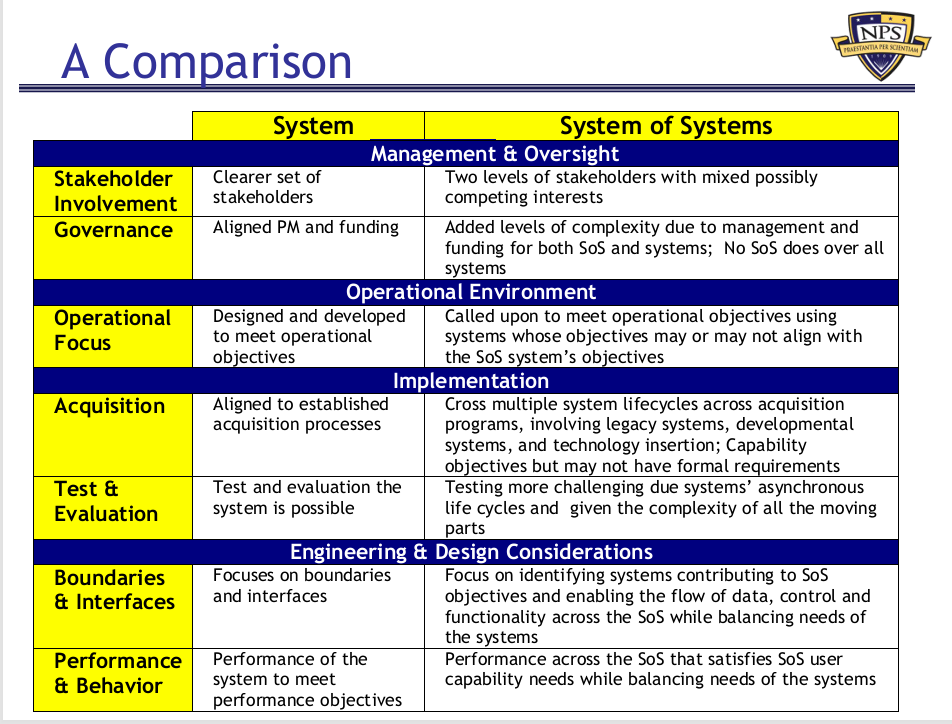
\includegraphics[width=0.5\linewidth]{figs/ch2/system-vs-sos.png}
    \caption{Enter Caption cite giachetti slides}
    \label{fig:placeholder}
\end{figure}

Lifecycle perspective: concept → development → production → operations → retirement 
discuss multiple lifecycle styles -- vee, spiral, etc...

A System of Systems is “a set or arrangement of systems that results when independent and useful systems are integrated into a larger system that delivers unique capabilities.” [OSD Systems Engineering Guide for Systems of Systems, August 2008]

SoS characteristics -- pull from Maier book

SoS engineering approach and how to manage it \cite{vaneman_defining_SoS_2013}

Emergent properties: system behaviors that arise from component interactions, not predictable from individual parts alone. changes propagate across subsystems, creating ripple effects-- cite 4950 documentation from giachetti

Scale challenges: modern systems (aircraft, spacecraft, infrastructure) involve thousands of requirements and components. find an example to deoonstrate the complexity. NASA docs? F35 or other fighter jets? Automobiles?

Standards context: ISO/IEC/IEEE 15288, INCOSE Systems Engineering Handbook

\subsection{Document-Centric vs. Model-Centric Workflows}\label{subsec:mbse}

%---------------------- DOCUMENT CENTRIC PORTION -----------------
Traditional document-centric: requirements in text documents, specifications in PDFs, manual traceability matrices
Document-centric limitations: version control difficulties, inconsistency across artifacts, manual updates, limited automated analysis

pull from Introduction To Model-Based System Engineering (MBSE) and SysML by Laura hart.

%---------------------- MBSE CENTRIC PORTION -----------------
MBSE definition: formalized application of modeling to support system requirements, design, analysis, verification throughout lifecycle

\ac{mbse} is defined by the \ac{sebok} as "a paradigm that uses formalized representations of systems, known as models, to support and facilitate the performance of \ac{se} tasks throughout a system’s life cycle" \cite{incose_guide_2025}

MBSE benefits: single source of truth, automated consistency checking, improved traceability, stakeholder communication
Modeling languages: SysML, UAF, OPM as formal representations (cite OMG standards)
Modeling frameworks: Business processes, DODAF, UAF, etc...
MBSE tools: Cameo Systems Modeler, MagicDraw, Capella, others (cite vaneman study that he published this year) 

Transition challenges: organizational inertia, training requirements, tool costs, legacy integration
Hybrid reality: most organizations operate with mixed document/model approaches 


\subsection{Opportunities for AI and Large Language Models in Systems Engineering}\label{subsec:ai_opportunities}

Provide examples of typical SE tasks such as requirements analysis, trade-space exploration, and risk management. Outline current and potential uses of LLMs in SE toolchains (e.g., MBSE, traceability, decision support).

consensus methods (cite some of the work i did along with other classical consensus methods found in my nps ars paper) 

\subsection{Foundational Capabilities, Failure Modes, and Limitations of Language Models}\label{subsec:llm_foundation_failure_limitations}

\subsubsection{Foundational Capability}
% -------------- FOUNDATIONAL CAPABILITY  --------------
LLM architecture: transformer-based models trained on massive text corpora
Core capabilities: natural language understanding, generation, reasoning, few-shot learning
Scale effects: emergent abilities appearing in larger models (e.g., chain-of-thought reasoning)

Large Language Models (LLMs) are neural networks that have revolutionized the field of natural language processing (NLP) by demonstrating an impressive ability to understand and generate text. Many models have also demonstrated an ability to generate code in common languages (e.g. Python).

Training: Teaching a model how to perform a task using large amounts of data

Inferencing: Model making inferences based on new inputs

Common LLMs (not an exhaustive list)
Proprietary: OpenAI ChatGPT, Google Gemini, Anthropic Claude
Open source: Llama, Falcon, Mistral

Model Characteristics 
Size is the number of parameters (e.g. 70B model = 70B parameters)
Quantization is a compression technique used to reduce memory and compute requirements. It converts weights to a lower precision data type (e.g. 32 bit floating point, 16float, 8 or 4 bit integer).

<< inisert ai and gen ai png?? >>

AI, Language Models, Improving Responses
Re-Training: Re-train base model with new dataset
Finetuning: Teach the base model specialized knowledge by adjusting a small number of internal parameters. Significant time savings compared to re-training entire model
Retrieval Augmented Generation (RAG): Utilize external data to augment the LLM’s knowledge without changing model weights
Prompt Engineering: Optimize prompts for optimal outputs
Few Shot prompts teach LLMs to perform a task through examples (Oleszak, 2024)
Zero Shot prompts challenge the LLM to perform a task correctly when it has not been correctly trained for that task
These methods can be combined.

temperature Consider having a shrot section on temperature. Something that leverages something like the image below.
% \begin{figure}[htbp]
%     \centering
%     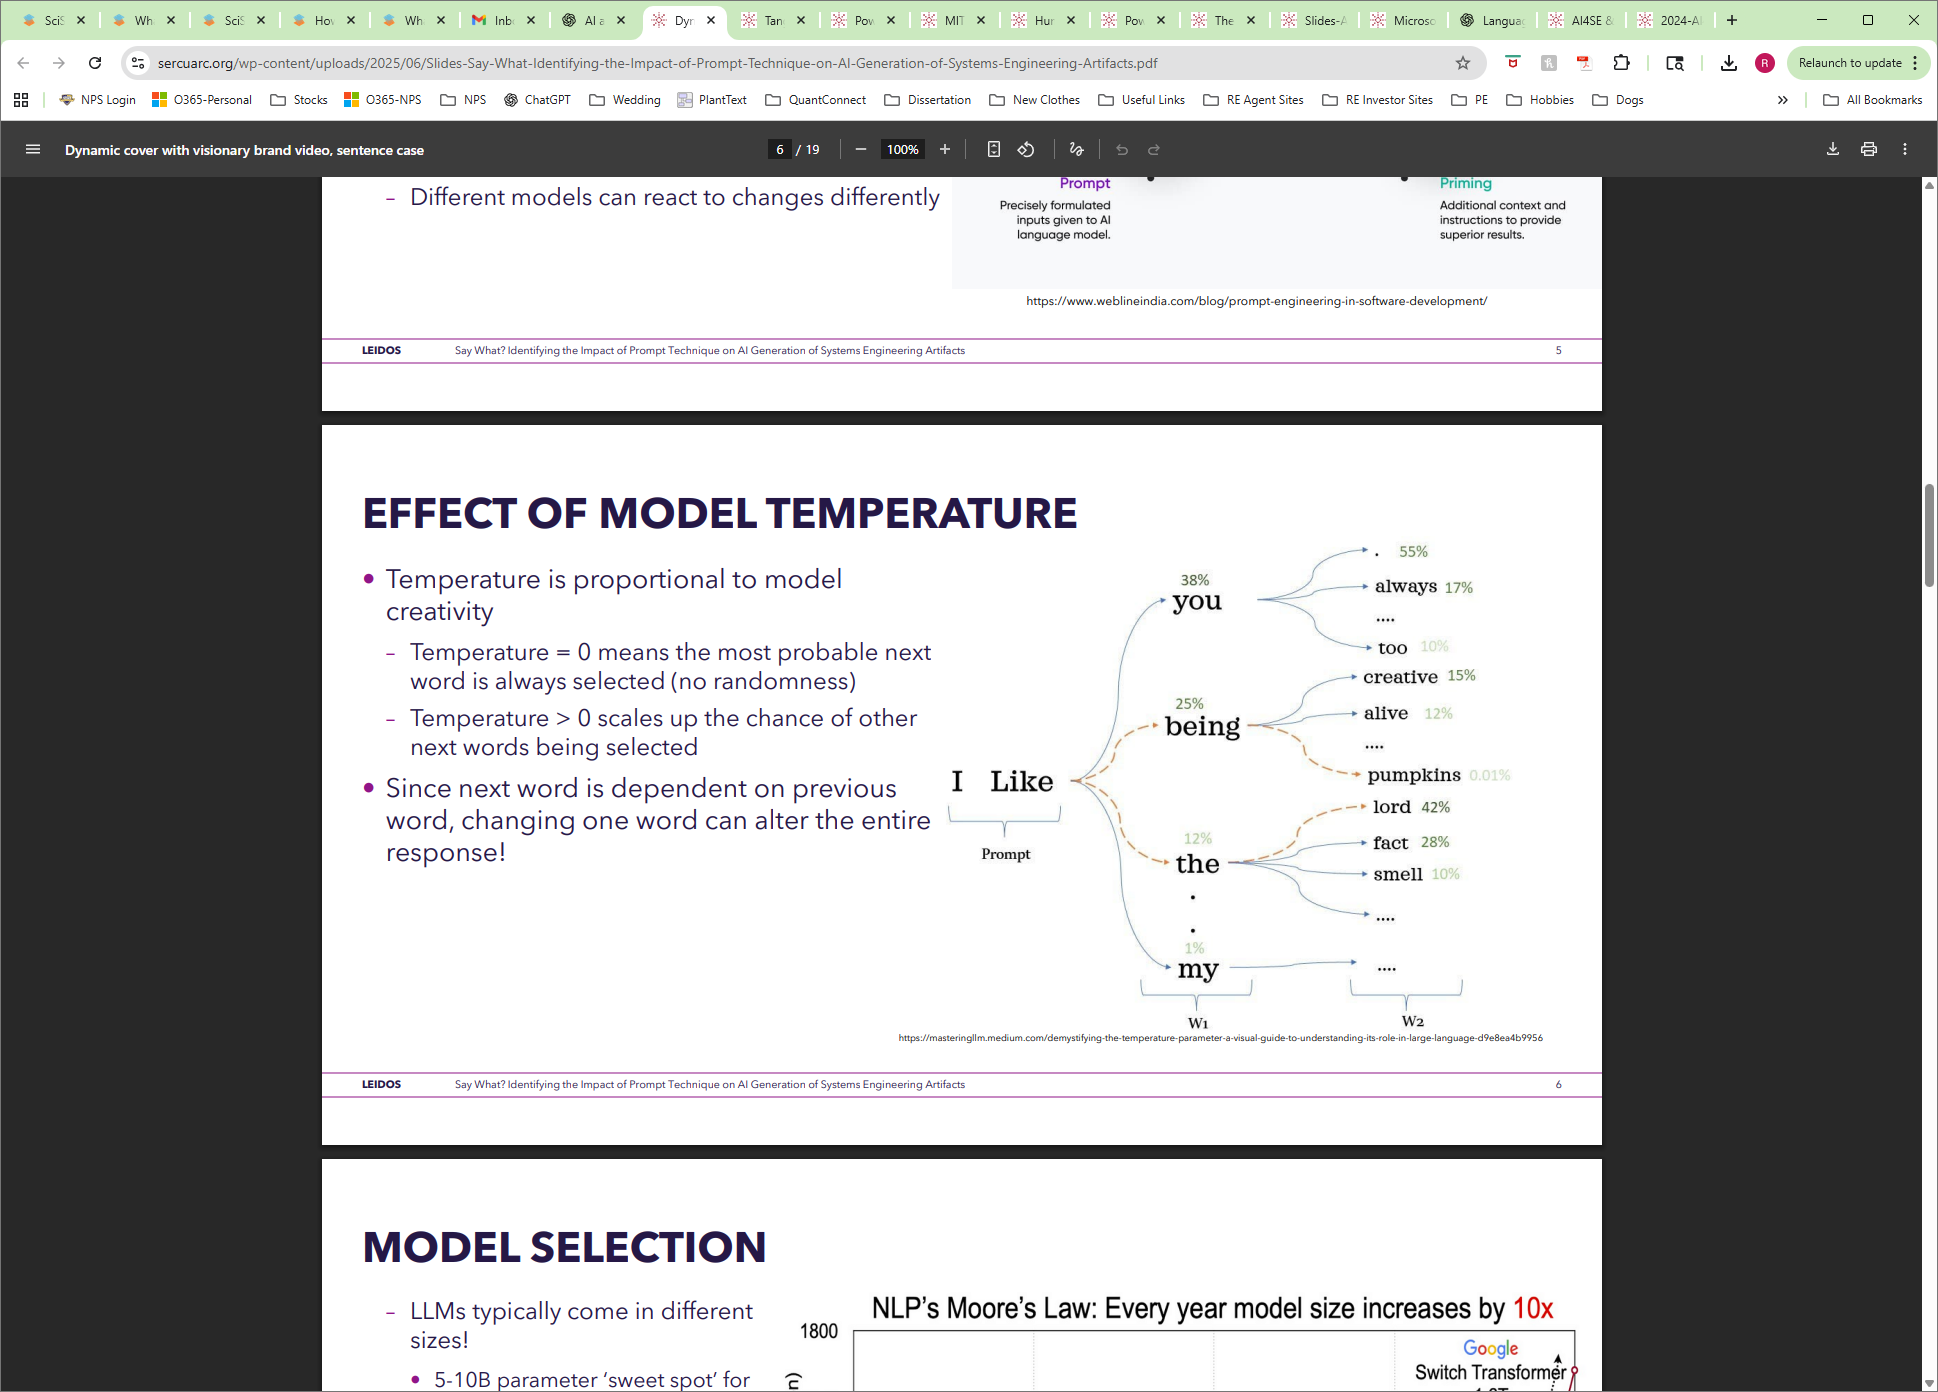
\includegraphics[width=0.8\textwidth]{figs/ch2/2.3/temperature-explaination.png}
%     \caption{Placeholder}
%     \label{fig:temperature-explaination}
% \end{figure}

add in a discussion about  vision and spatial models (for spatial models reference, see the rundown ai email on gmail which references AI specalist DR> Fei-Fei and here new published essay on spatial intelligence. Make sure the reader understand the scope for this manuscript is textual only.


% -------------- FAILURE MODES  --------------
\subsubsection{Failure Modes}
Hallucinations: generating plausible but factually incorrect or fabricated information
Training data contamination: test set leakage or memorization affecting evaluation validity
Grounding failures: lack of connection to real-world physics, causality, or domain constraints
Prompt injection: adversarial inputs that override intended behavior or safety constraints
% -------------- LIMITATIONS --------------
\subsubsection{Limitations}
Context window limitations: finite memory affecting long document processing
Inconsistency: different outputs for semantically equivalent prompts -- DISCUSS TEMPERATURE
Lack of uncertainty quantification: confident-sounding outputs regardless of actual knowledge
Domain specificity: general pre-training may not capture specialized knowledge
Safety-critical gap: difference between "usually correct" and "provably correct" for critical systems


Discuss the new 3D spatial models is the next frontier cite press conference, new spatial model publication

% ------------------------------------------------------------------------------

\section{Benchmarking Language Models: Foundations, Modalities, and Gaps}\label{sec:benchmarking}

\subsection{Foundations of Benchmarking in AI}\label{subsec:benchmarking_foundations}
% What benchmarks are for
% Historical evolution: MNIST → GLUE → MMLU → BIG-Bench

\subsubsection{Benchmarking Nomenclature}
Benchmark:
A set of inputs (prompts, questions, documents) with ground-truth outputs and a protocol that defines how the model should interact with them.
Examples: 
Multitask Multiple Choice (MMLU)
Grade-School Math (GSM8K)
Metric:
A formula that turns the model’s outputs on a task into a number (score).
Examples: 
Bilingual Evaluation Understudy (BLEU)
Recall-Oriented Understudy for Gisting Evaluation (ROUGE)

Takeaway:
A task is what the model is asked to do; a metric is how we measure whether it did it well.

<< add the benchmarking taxonomy figure >>

This figure includes meta-evaluations (which is essentially what this dissertation is).

mention how we evaluate at a temperature=0 to make it deterministic.


\subsubsection{Dataset Creation, Saturation, and Deprecation}\label{subsubsec:dataset_lifecycle}
% How benchmarks are built
% Why they saturate
% Dangers of contamination
% Concept drift and lifecycle of benchmarks
% Why new benchmarks emerge as capabilities evolve
Discuss dataset creation practices and constraints that affect benchmark validity.


\subsection{General Benchmark Frameworks and Evaluation Tools}\label{subsec:benchmark_tools}
% LM-Eval-Harness, HELM, BenchBuilder, HF Evaluate, evaluation strategies, implementation differences
% (Pull content from your prior papers)


\subsection{Evaluation Modalities for LLM Performance}\label{subsec:evaluation_modalities}

\begin{itemize}
    \item Strategies for selecting representative benchmark questions, creating training/validation/test splits, and avoiding data leakage.
    \begin{itemize}
        \item Selecting benchmark questions
        \item creating training/validation/test splits
        \item avoiding data leakage
    \end{itemize}
    \item Outline conventional evaluation metrics used in LLM research (accuracy, F1, BLEU, etc.). ROUGEL
    \item Detail multiple-choice question (MCQ) evaluation: design principles, scoring methods, and diagnostic power.
    \item Present open-style question (OSQ) evaluation: rationale, metrics, and grading complexity.
    \begin{itemize}
        \item regular osq metrics? rubrics?
        \item LLM-as-a-judge
    \end{itemize}
    \item Compare MCQ and OSQ approaches, highlighting trade-offs in objectivity, conceptual depth, and cost.
    \item Show how these modalities support the measurement of reasoning and conceptual understanding in SE tasks.
\end{itemize}

\subsubsection{Multiple-Choice Question (MCQ) Evaluation}\label{subsubsec:mcq_eval}

% MCQ variance / resilient MCQ sources
% Making good MCQA benchamrks, protecting against adversarial distractors
\cite{yigit_adversarial_2025}
This research emphasizes the need to evolve model evaluation practices. Traditionally, MCQA systems have been evaluated based only on their ability to select the correct answer. However, the study suggests that evaluation frameworks should incorporate performance under adversarial conditions as well. By integrating adversarial distractor generation into model testing pipelines, researchers and practitioners can more thoroughly diagnose system vulnerabilities.

Similar to \cite{ghanem_DISTO_2023} -- how to create good distractors.

Similar problems in Visual MCQs where choice selected without the model reading them \cite{zhang_mitigating_2025}




% Strengths/weaknesses, distractor sensitivity, position bias
\acp{mcq} have long been a mainstay in educational and professional assessments due to their simplicity and objectivity. In the context of evaluating \acp{llm}, \acp{mcq} offer a straightforward testing mechanism: a model selects from a finite set of answers, making it easy to measure correctness. The \ac{mcq} format provides a quantifiable snapshot of a model’s baseline knowledge and pattern-recognition abilities.

However, \acp{mcq} inherently conceal the complexity of the reasoning processes that can be assessed, meaning they offer little insight into how or why a model arrived at a particular choice. For systems engineering, the how or why is critical to evaluating competing trade-spaces and picking a solution that balances competing interests. 

By constraining possible answers, \acp{mcq} may oversimplify complex topics. Systems engineering scenarios that require in-depth reasoning, synthesis of multiple concepts, or consideration of subtle trade-offs are not easily captured by a handful of fixed options. This lack of nuance means MCQs may not truly reflect the model’s capacity for deep understanding or its ability to articulate reasoning processes \cite{zheng_large_2024, fu_mcq_reasoning_more_confident_when_wrong_2025}. In complex engineering environments, relying solely on MCQs risks obtaining an incomplete picture of the model’s actual capabilities. Recent research suggests that providing \acp{llm} with no correct \ac{mcq} can assist in measuring reasoning and critical thinking \cite{goral_when_all_options_are_wrong_2024}.

Textual response formats challenge LLMs to generate answers in free form, demanding a richer comprehension of the underlying material. By forgoing multiple-choice constraints, these formats encourage models to articulate reasoning, structure their responses coherently, and demonstrate the ability to connect concepts holistically. For instance, a prompt might ask the LLM to explain how a particular subsystem interacts with other components or to propose a solution that balances performance and cost.

The advantage of textual responses lies in their ability to reveal more about the model’s internal “thought process” as demonstrated by reasoning models like ChatGPT o1 or DeepSeek R1 \cite{IntroducingOpenAIO1_2024, deepseekai_deepseekR1-2025}. Evaluating free text answers can uncover subtle reasoning errors or expose areas where the model lacks conceptual depth. While more complex to assess automatically, textual response evaluation could be aided by sophisticated metrics or even human expert review.

Despite their merits, textual responses pose significant practical challenges. Creating a dataset of open-ended questions is often more involved than formulating MCQs. It requires careful thought to ensure that prompts are unambiguous and representative of real-world tasks, while maintaining a relatively tightly bounded question. Since textual responses are not strictly right or wrong in the same way MCQ choices are, developing reliable evaluation metrics is complex. Traditional measures like accuracy scores do not directly apply. The model might produce grammatically correct but conceptually vacuous answers or resort to vague generalities that sound authoritative but lack technical rigor \cite{fu_mcq_reasoning_more_confident_when_wrong_2025,Sourav_Banerjee_2024_Vulnerability_LLM_Benchmarks}. Addressing these challenges will involve combining automated metrics with domain expert human evaluation. 

\subsubsection{Open Style Question and Free-Response Evaluation}\label{subsubsec:osq_eval}
% Conceptual reasoning, rubric-based judging, human scoring, LLM-as-judge


% LLM as a judge




below is from page 5 of "LLMs-as-Judges: A Comprehensive Survey on LLM-based Evaluation Methods" by haitao li. Snag the diagram before this one too. It was good.
\begin{figure}
    \centering
    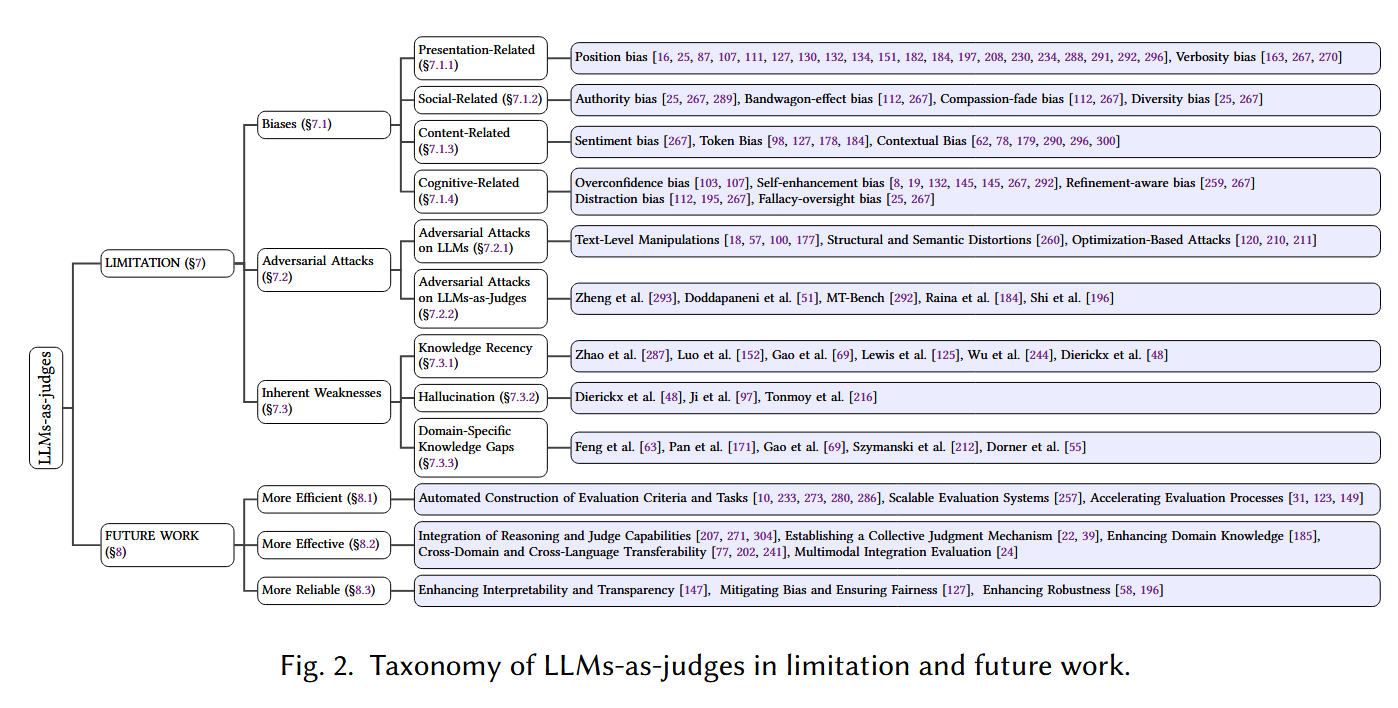
\includegraphics[width=1\linewidth]{figs/ch2/taxonomy-of-llm-as-judge-limitations.png}
    \caption{Enter Caption add citation "LLMs-as-Judges: A Comprehensive Survey on LLM-based Evaluation Methods" by haitao li}
    \label{fig:placeholder}
\end{figure}


\begin{figure}
    \centering
    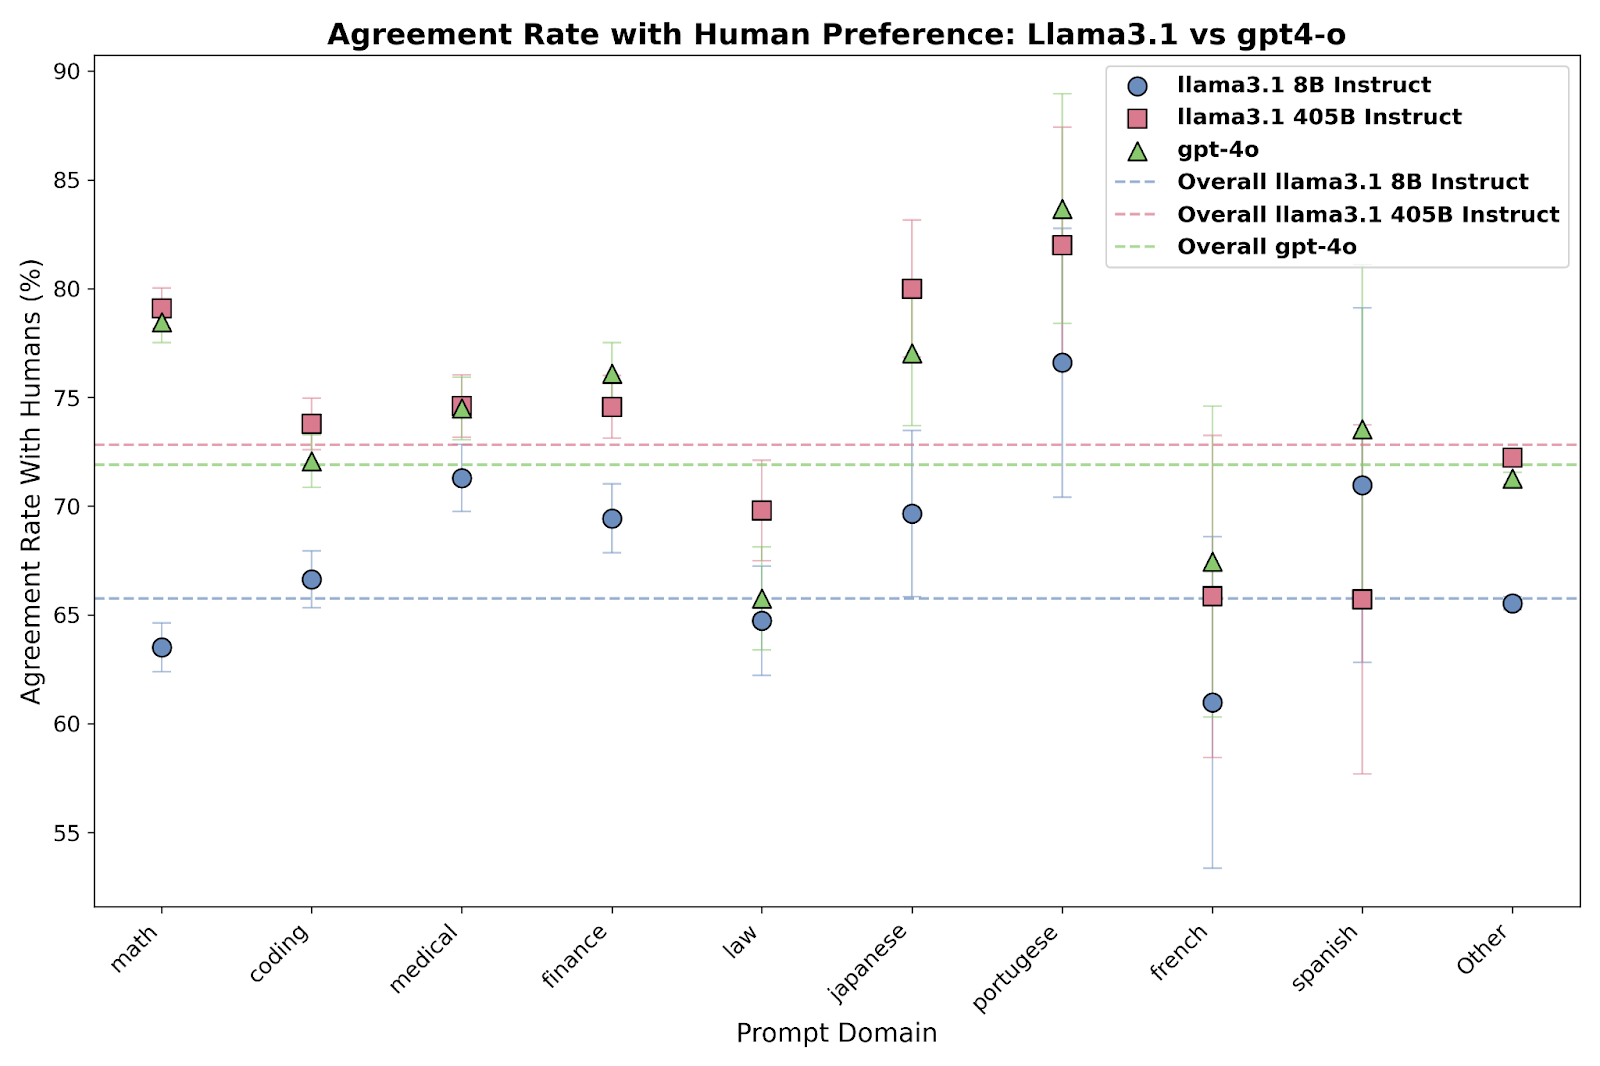
\includegraphics[width=0.5\linewidth]{figs//ch2/llm-agreement-rate.png}
    \caption{Agreement Rate between LLM Judges and Human Preferences by Domain from Chatbot Arena <cite the 9 and 9 from website below}
    \label{fig:placeholder}
\end{figure}

% the website to cite this from
https://sambanova.ai/blog/can-llama-405b-outperform-gpt4?
https://huggingface.co/datasets/lmarena-ai/arena-human-preference-55k
https://lmarena.ai/

\subsection{Current Benchmarking Landscape}\label{subsec:benchmark_landscape}


\subsubsection{General Knowledge Benchmarks}\label{subsubsec:general_benchmarks}
% MMLU, BIG-Bench, GPQA, MSG, Arena-Hard, etc.
Review major general-purpose LLM benchmarks (e.g., MMLU, HELM), their objectives, and their limitations for SE.

discuss textual benchmarks vs some vision vs spatial benchmarks for a paragraph.
mention Sudoku bench as a spatial benchmark. (Launched May 2025). A quote may be "67\% of the puzzles remained unsolved as models struggle with meta-reasoning (learning novel rules and creative "break-in" as this source describes it. Find the paper and see if that's the proper quote.


\subsubsection{Domain-Specific Benchmarks}\label{subsubsec:domain_benchmarks}
% Medical, biomed, legal, finance
% Cross-domain strategies and lessons for SE

Introduce SysEngBench as a domain-specific benchmark mapped to INCOSE concepts and explain how it addresses gaps in generic benchmarks.

\subsubsection{Unique Evaluation Challenges in Systems Engineering}\label{subsec:se_eval_challenges}
% SE task types, reasoning depth, MBSE semantics, trade-space analysis

Introduce SysEngBench as a domain-specific benchmark mapped to INCOSE concepts and explain how it addresses gaps in generic benchmarks. And how it provides an extensible framework

\begin{itemize}
    \item Describe how SE’s multidisciplinary, life-cycle–oriented tasks differ from typical NLP benchmarks. Or how can we conform to a more complex benchmark like ARC42 or similar.
    \item Explain challenges in capturing abstract reasoning, trade-offs, and multi-stakeholder requirements.
    \item Discuss the difficulty of representing SE-specific terminology and model-based representations (e.g., SysML) in benchmarks.
    \item Address domain-specific concerns such as safety, reliability, and regulatory compliance.
    \item Highlight lessons from domain-specific benchmarks in fields such as biomedical, legal, and finance to inform SE benchmarking.
\end{itemize}

% ------------------------------------------------------------------------------

\section{Cost Modeling and Tokenomics}\label{sec:cost_modeling_tokenomics}
Cost estimation has long been a central concern in systems engineering, and it provides
useful context for understanding emerging economic considerations of large language models (LLMs).  
Key themes from the literature include:

\subsection{Established SE Cost-Modeling Foundations}

\begin{itemize}
    \item The \ac{cocomo} model \cite{boehm_cocomo_1981} estimates software development cost using size, complexity, and personnel factors.
    \item The \ac{cosysmo} model \cite{valerdi_cosysmo_2005} extends these ideas to systems engineering projects, accounting for system-of-systems complexity and integration effort.
    \item Other approaches such as SEER, PRICE, and hybrid parametric–analogy models broaden cost estimation methods \cite{madachy_systems_2024, madachy_cost_estimation_2014}.
\end{itemize}

\subsection{Emergence of Tokenomics Cost Modeling for Language Models}

\begin{itemize}
    \item LLM-supported tasks incur usage-based costs tied to token counts, model size, and inference latency.  
    \item Tokenomics refers to measuring and analyzing these computational and economic trade-offs, including aggregate and per-query token counts, throughput, and runtime to estimate costs (e.g., \$/million tokens).
    \item Understanding tokenomics is essential for assessing the scalability and affordability of AI-assisted systems engineering.
\end{itemize}



